\documentclass[tikz,border=8pt]{standalone}
\usepackage{pgfplots}
\pgfplotsset{compat=1.18}

\definecolor{navy}{HTML}{1F2D3D}
\definecolor{blue}{HTML}{2F6FB0}
\definecolor{orange}{HTML}{E08A3C}
\definecolor{lightblue}{HTML}{C9D7E6}
\definecolor{gridc}{HTML}{DFE6EE}

\begin{document}
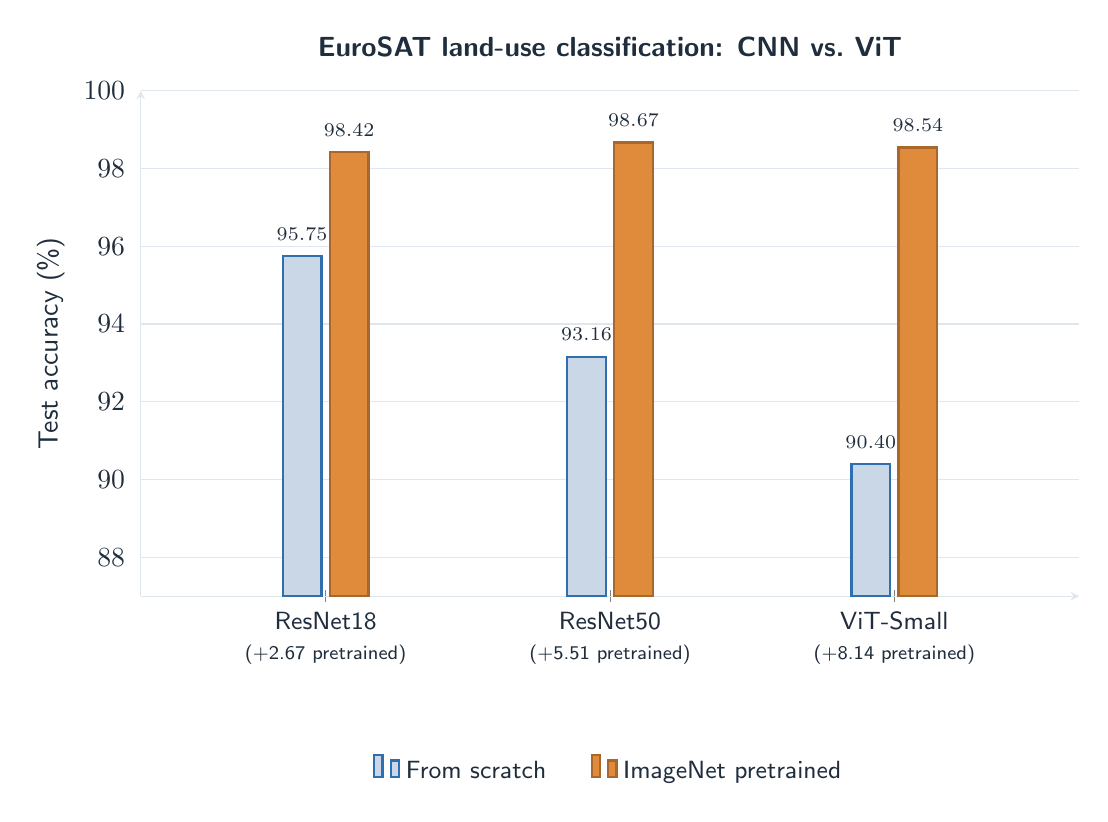
\begin{tikzpicture}
\begin{axis}[
  width=13.5cm, height=8cm,
  ybar=3pt, bar width=14pt,
  xmin=0.35, xmax=3.65,
  ymin=87, ymax=100,
  ylabel={\sffamily Test accuracy (\%)},
  ylabel style={text=navy},
  xtick={1,2,3},
  xticklabel style={text=navy, font=\sffamily\small, align=center},
  xticklabels={
    {ResNet18\\{\scriptsize(+2.67 pretrained)}},
    {ResNet50\\{\scriptsize(+5.51 pretrained)}},
    {ViT-Small\\{\scriptsize(+8.14 pretrained)}}
  },
  ytick style={draw=none},
  yticklabel style={text=navy},
  ymajorgrids=true,
  grid style={gridc},
  axis lines=left,
  axis line style={gridc},
  nodes near coords={\pgfmathprintnumber[fixed,precision=2,zerofill]{\pgfplotspointmeta}},
  nodes near coords style={font=\sffamily\scriptsize, text=navy, yshift=2pt},
  title={\sffamily\bfseries EuroSAT land-use classification: CNN vs.\ ViT},
  title style={text=navy, yshift=3pt},
  legend style={draw=none, fill=none, font=\sffamily\small, text=navy,
                at={(0.5,-0.30)}, anchor=north, legend columns=2,
                /tikz/every even column/.append style={column sep=14pt}},
  legend cell align=left,
]
\addplot[fill=lightblue, draw=blue, line width=0.8pt]
  coordinates {(1,95.75) (2,93.16) (3,90.40)};
\addlegendentry{From scratch}
\addplot[fill=orange, draw=orange!75!black, line width=0.8pt]
  coordinates {(1,98.42) (2,98.67) (3,98.54)};
\addlegendentry{ImageNet pretrained}
\end{axis}
\end{tikzpicture}
\end{document}
